\selectlanguage{english}
\begin{abstract}
    \noindent For the second project of the Computer Simulations (ELTE Physics MSc) course I propose the concept of a molecular dynamics simulation, using the velocity Verlet integration. I intend to also implement Verlet's pair-list method, along with his Lennard-Jones potential cut-off method. It is also planned, to make the simulation with both periodic and closed boundary conditions. In the second case, if a molecule hits the wall, it will bounce of with a completely flexible collision.
\end{abstract}

\begin{multicols}{2}
\section{Introduction}
The aim of molecular dynamics simulations are to make it possible to effectively study the thermodynamic parameters of fluids. Using our current technology it is not possible yet to simulate the microscopic behaviour of the particles of a macroscopic system. Our goal should be to create such a simulation, where the examined parameters could be measured even using very small number of particles. \par
The method which will be used here was introduced by Loup Verlet in his notorious paper \citep{verlet1967computer}. Along with the numerical corrections proposed by also him, this type of algorithm could be used to simulate a molecular system $10$ times faster, than the Runge-Kutta method.

\section{Motivation}
Since I've run out of time during the making of the previous project, I decided to do a more simple, but still interesting and visually appealing simulation. Last year I've already tried 

\section{Description of the proposed assignment}
In this project I will build a molecular dynamics simulation, using the Velocity-Verlet integration. As a reasonable approximation for the interaction between the particles, I'm going to use the Lennard-Jones potential, which is often used in the approximate description of the interaction between a pair of neutral atoms or molecules. \par
Since this potential is short-ranged, the effect of the distant particles could simply ignored outside an $r_{c}$ cut-off distance, thus creating a so-called "truncated and shifted Lennard-Jones potential". This cut-off distance is usually chosen to be $r_{c} = 2.5 \sigma$ \citep{2011JChPh.134h1102T}, where $\sigma$ is the finite distance at which the Lennard-Jones potential is zero. In conclusion, when calculating the forces acting on a single particle, instead of calculating the effect of every molecule, we calculate the forces from those particles only, which are situated within a sphere of $r_{c}$ radius around our central one. \par
It is also advised to implement Verlet's pair-listing method to speed up the simulation. If we first select all of the particles inside an $r_{c}$ radius around a single particle at every step, the simulation would be still very slow, because it is an $\mathcal{O} \left( N^{2} \right)$ hard problem. To solve this, we define a sphere around every particle with $r_{\text{max}} > r_{c}$ radius, and we call the list of every particle inside the $i$th sphere the pair-list of the $i$th particle. If during the calculation of forces acting on the $i$th particle we only need to loop through its neighbours inside the $i$th pair-list, without the need of selecting nearby ($r < r_{c}$) particles at every step. Since microscopic objects move at a finite speed, it is trivial that if we choose $r_{\text{max}} > r_{c}$, we only need to update this list only after every few step, because the interacting particles need a finite amount of time to move out from it. The standard value of $r_{max} = 3.2 \sigma$ usually.

\section{Theoretical background}
\subsection{Verlet and velocity Verlet algorithm}
The advisedly used algorithm (velocity Verlet method) is a variation of the somewhat simpler Verlet method. Both of them have their pros and cons. While the Verlet method's accuracy ($\mathcal{O} \left( \tau^{4} \right)$) approaches the Runge-Kutta's ($\mathcal{O} \left( \tau^{5} \right)$), it can't be started from a single initial position, since its stepping rule uses the $n$th and $(n-1)$th positions and velocities to calculate the $(n+1)$th values. The stepping rule is the following:

\begin{equation}
\vec{R}_{n+1}
=
2 \vec{R}_{n} - \vec{R}_{n-1} + \tau^{2} \vec{A}_{n} + \mathcal{O} \left( \tau^{4} \right)
\end{equation}
\begin{equation}
\vec{V}_{n+1}
=
\frac{\vec{R}_{n+1} - \vec{R}_{n-1}}{2 \tau} +  \mathcal{O} \left( \tau^{2} \right)
\end{equation}
Here $\vec{R}$ denotes the coordinate vector and $\vec{V}$ denotes the velocity vector of a particle, $\tau$ is the step size of the simulation. Another disadvantage of the Verlet method, that for the $\vec{V}$ propagation its accuracy is only $\mathcal{O} \left( \tau^{2} \right)$. \par
In contrast the velocity Verlet method could be started from an arbitrary initial position. Its stepping rule is the following:

\begin{equation}
\vec{R}_{n+1}
=
\vec{R}_{n} + \tau \vec{V}_{n} + \frac{\tau^{2}}{2} \vec{A}_{n} + \mathcal{O} \left( \tau^{3} \right)
\end{equation}
\begin{equation}
\vec{V}_{n+1}
=
\vec{V}_{n} + \frac{\tau}{2} \left( \vec{A}_{n+1} + \vec{A}_{n} \right) + \mathcal{O} \left( \tau^{3} \right)
\end{equation}
If we only want to accurately measure the conservation of energy and the coordinates of the molecules, we can combine the two method, where the first two step is evaluated by the velocity Verlet method, and the following are with the Verlet method. Here I will use only the velocity Verlet method for the whole simulation.

\subsection{Lennard-Jones potential}
The interaction between chargeless atoms or molecules could be approximated the already mentioned Lennard-Jones potential:

\begin{equation}
V^{LJ} \left( r \right)
=
4 V_{0} \left[ \left( \frac{\sigma}{r} \right)^{12} - \left( \frac{\sigma}{r} \right)^{6} \right]
\end{equation}
Here $\sigma$ is the already mentioned, finite distance, where the Lennard-Jones potential becomes zero. $V_{0}$ is the absolute value of the potential's value at the minimum ($V_{0} = \left| V_{min} \right|$). The reason to write the equation in this form could be easily understood. The $r^{-12}$ term is comes from the Pauli exclusion principle, which creates a significantly strong repulsion between the particles if they're very close to each other. On larger ranges the Van der Waals force overcomes this repulsion, and exert an attractive force on the molecules, thus adding the $r^{-6}$ term into the equation with a negative sign. At a characteristic distance $r_{m} = 2^{1/6} \sigma$ the potential reaches it's minimum value ($-V_{0}$), where the attraction is the strongest. Further increasing the distance between the particles, this attraction slowly decreases. \par
\begin{center}
	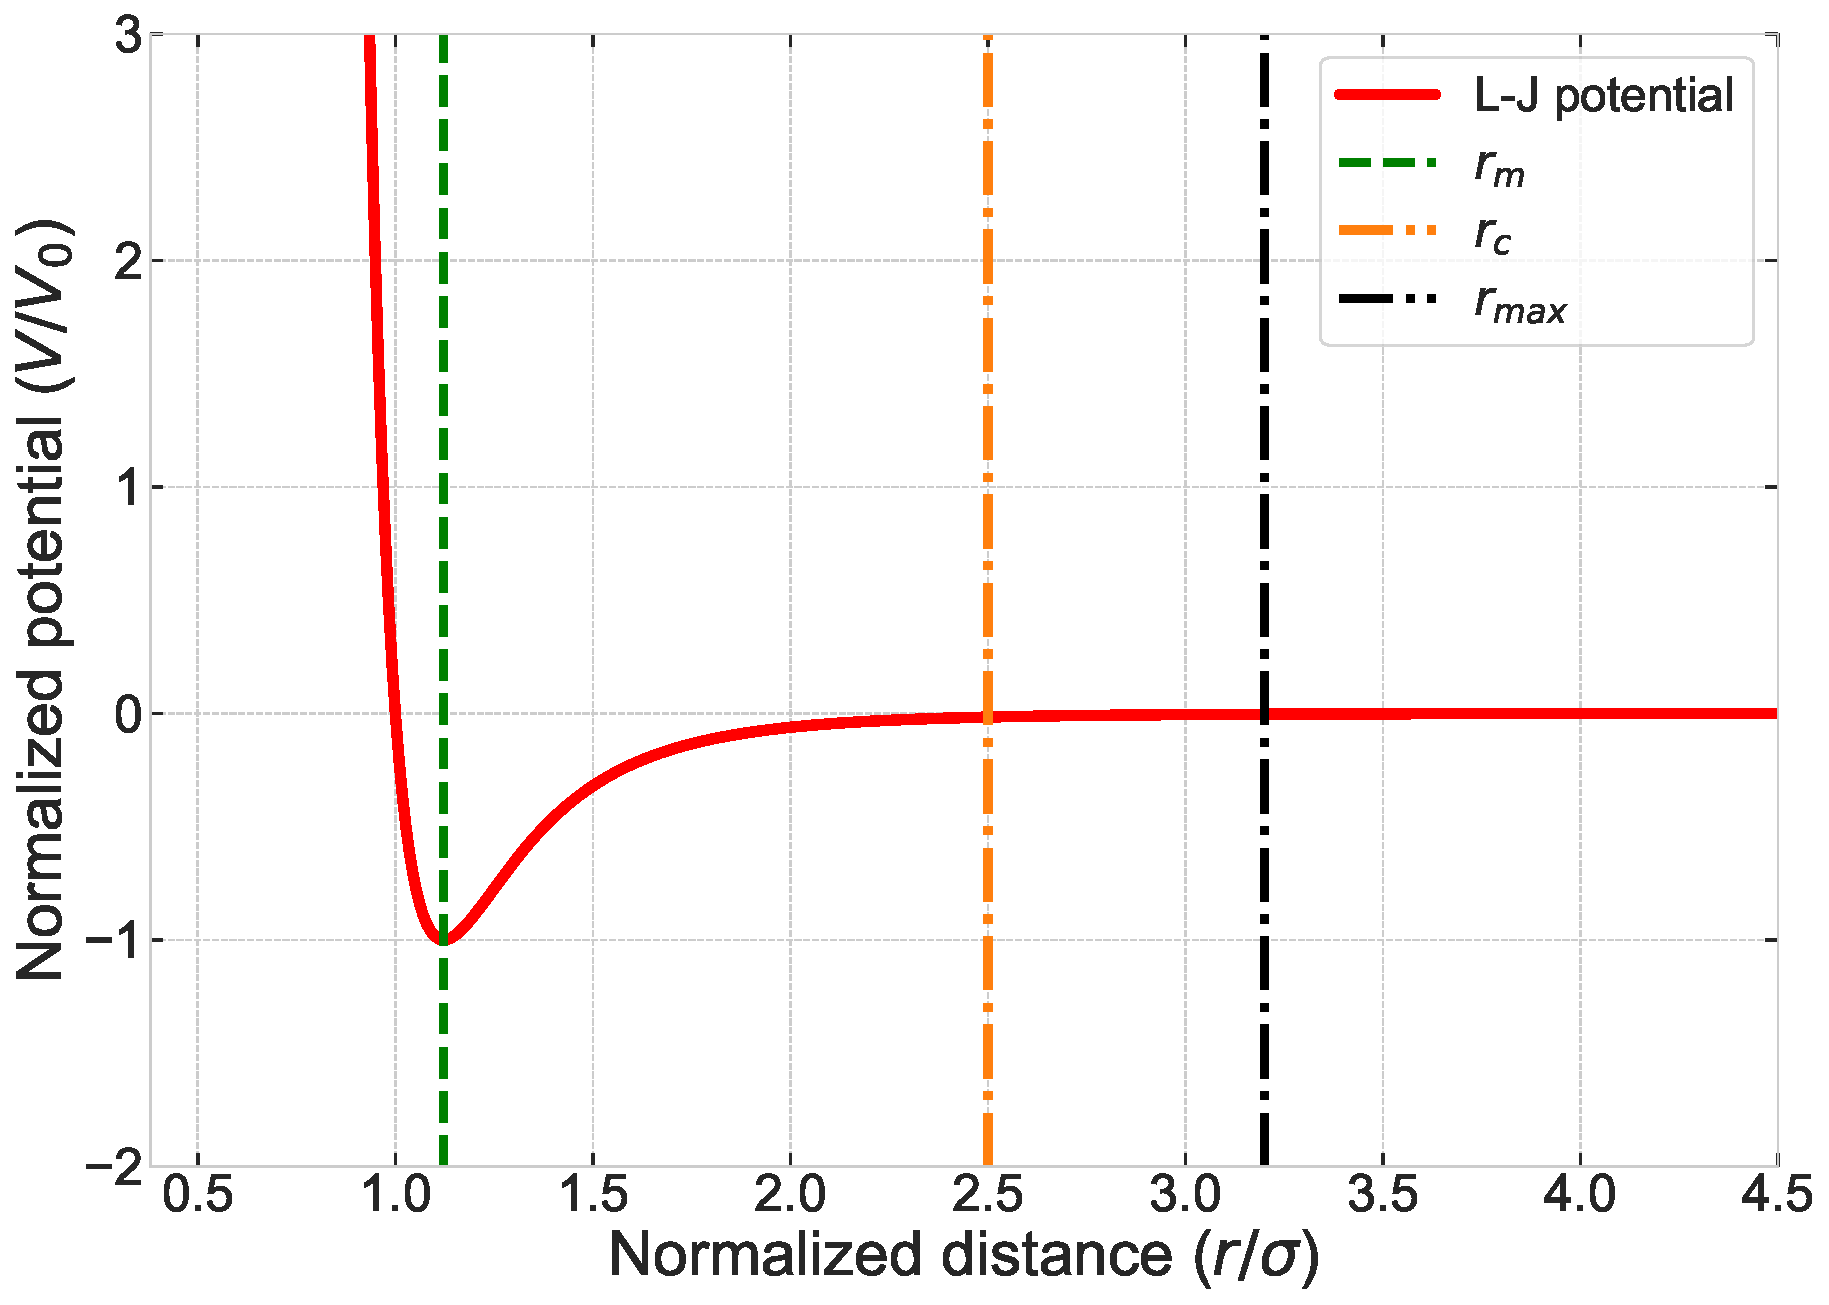
\includegraphics[width=0.5\textwidth]{img_src/Lennard_Jones_Potential.pdf}
	\captionof{figure}{The Lennard-Jones potential} \label{fig:2}
\end{center}
The force, which is used to calculate the accelerations for the stepping rules could be given by calculating the gradient of the potential:

\begin{equation}
\vec{F} \left( r \right)
=
-\boldsymbol{\nabla} V^{LJ} \left( r \right)
=
\frac{24 V_{0}}{r^{2}} \left[ 2 \left( \frac{\sigma}{r} \right)^{12} - \left( \frac{\sigma}{r} \right)^{6} \right] r
\end{equation}
Using the cut-off method the Lennard-Jones potential becomes zero at $r \leq r_{c}$. Thus the truncated and shifted Lennard-Jones potential is the following:

\begin{equation}
V_{tf}^{LJ} \left( r \right)
=
\begin{cases}
4 V_{0} \left[ \left( \frac{\sigma}{r} \right)^{12} - \left( \frac{\sigma}{r} \right)^{6} \right] & \text{if}\ r < r_{c} \\
0 & \text{if}\ r \leq r_{c}
\end{cases}
\end{equation}

\end{multicols}